\documentclass[11pt,twocolumn]{article}
\usepackage[plain]{algorithm}

\usepackage[brazil,english]{babel}
\usepackage[utf8]{inputenc}
\usepackage[T1]{fontenc}

\usepackage{graphicx,url}
\usepackage[hang]{subfigure}
\usepackage{psfrag}
\usepackage{url}
%\usepackage{hyperref} -- Deixa destacado as referências
\usepackage{cite}


\usepackage[a4paper,top=2cm,left=2cm,right=2cm,bottom=2cm]{geometry}

\usepackage[labelsep=endash]{caption}
\addto\captionsenglish{\renewcommand{\figurename}{Figura}}
\addto\captionsenglish{\renewcommand{\refname}{Referências}}

\sloppy

\begin{document}

\thispagestyle{empty}
\twocolumn[
\begin{center}
  \textbf{\Large Modelagem e Implementação em FPGA da Codificação 8b/10b}
\end{center}

\begin{center}  
  \textbf{V. A. dos Reis$^\ast$, L. A. Ramalho$^\ast$, A. A. Shinoda$^\ast$ \\}
  $^\ast$UNESP, Ilha Solteira, Brasil\\
  Departamento de Engenharia Elétrica\\
  e-mail: victor.afonsoreis35@gmail.com
\end{center}
]

\noindent\textbf{Abstract} - \textit{ In high speed communications, where the reability is very important, the coding 8b10b is indicated. At digital communications, one of signal integrity issues is the synchronism between transmitter and receiver. A long sequence of logical levels, zeros (0's) or ones (1's), can cause a desynchronism in the transmission channel. At this work, modeling and implements a coding 8b/10b system, wich give a solution to the unbalanced 	bits, in the FPGA development kit of Xilinx (Kintex 7), through the hardware description language VHDL by the software Vivado\textsuperscript{TM}. By the implementation, was obtained a generic system for test of encodings described at VHDL, besides parameters of frequency, data rate and characteristics of transmission operation using the coding 8b/10b system}. 
\newline \textbf{Palavras-chave}: \textit{High Speed Serial Link, Codificação 8b/10b, VHDL, FPGA}.

\section{Introdução}

A complexidade e performance dos sistemas de comunicação evoluíram ao longo do tempo, o que facilitou com que em qualquer meio de transmissão os dados conduzidos pudessem sofrer distorções ou inferências causadas por problemas no canal de transmissão \cite{Borges}. 

Em altas frequências, problemas como a dessincronização do sistema e ruídos no canal de transmissão são relevantes na comunicação digital. A dessincronização entre o transmissor/receptor e a aparição de dados ruidosos são fatores limitantes na velocidade dos sistemas \cite{pra}. 

A codificação 8b/10b é uma técnica de codificação em blocos, o qual adiciona-se redundâncias de forma lógica em um bloco de (m) bits gerando um bloco de (n) bits. Este mapeamento possui algumas características próprias da codificação, o qual possibilita a verificação de possíveis erros na transmissão. Algumas codificações em blocos realizam um balanço DC no dado, portanto permite facilitar a sincronização entre o emissor e receptor por meio de circuitos externos. Codificações como por exemplo a 4b/5b , a 6b/8b, a 8b/10b, a 64b/66b e a 128b/130b utilizam esse método\cite{Fourouzan}.

O uso da codificação em blocos aumenta a qualidade do sistema, apesar de diminuir a taxa efetiva de dados transmitidos \cite{Berlekamp}. Dessa maneira, o desafio resume-se em torno da análise dos parâmetros de cada codificação, sendo capaz de fornecer uma solução de menor custo e que atenda os requisitos do sistema \cite{Franaszek}. Sendo assim, o objetivo deste trabalho é modelar e implementar em \textit{VHSIC Hardware Description Language} (VHDL) um sistema com a codificação 8b/10b, dentro de um kit de desenvolvimento em FPGA da Xilinx(Kintex 7 KC705). Através dessa implementação, é possível obter informações e parâmetros do sistema.

Pela análise parcial do sistema implementado em FPGA, foi possível obter características do comportamento da codificação quando esta é submetida a erros entre transmissor e receptor. A seção 2 ressalta a teoria, a modelagem em máquinas de estado e a ilustração de um sistema no FPGA da codificação 8b/10b. A seção 3 descreve a implementação no FPGA do sistema descrito em VHDL. A seção 4 conclui os resultados da implementação no FPGA do sistema da codificação 8b/10b.

\section{Materiais e métodos}

\subsection{A Codificação 8b/10b}

Os dados de 8 bits são mapeados em 10 bits, dessa maneira alguns dados de 10 bits com o mesmo número de bits 1's e 0's são usados como dados de controle da transmissão \cite{Franaszek}. Na codificação é descrito o conceito de disparidade, apresentando dois tipos: a disparidade do sistema, ou do inglês \textit{Running Disparity} (RD), e a disparidade dos dados. A disparidade é definida como a diferença entre o números de bits 1's e 0's do dado codificado para 10 bits. 

A codificação é descrita de forma que os dados transformados em 10 bits só possuam disparidade de dados +2, -2 ou 0 (nula). Desta maneira, a disparidade dos dados é obtida no momento em que se codifica o dado de entrada para 10 bits. A disparidade do sistema, ou RD, é obtida seguindo regras de acordo com a disparidade dos dados e também é responsável pela escolha dos dados no momento da codificação \cite{Franaszek}.

O RD alterna-se entre +1 e -1 ou permanece o mesmo, de acordo com as regras, das disparidades dos dados, ilustradas na Figura \ref{rd}. Quando o RD for -1 não é possível a disparidade dos dados ser -2, assim como se o RD for +1 é impossível a disparidade dos dados ser +2. Nestes casos, ao se obter esse tipo de disparidade para cada RD mencionado, no lado do receptor, representa-se um erro na transmissão.

\begin{figure}[htb]
	\centering
	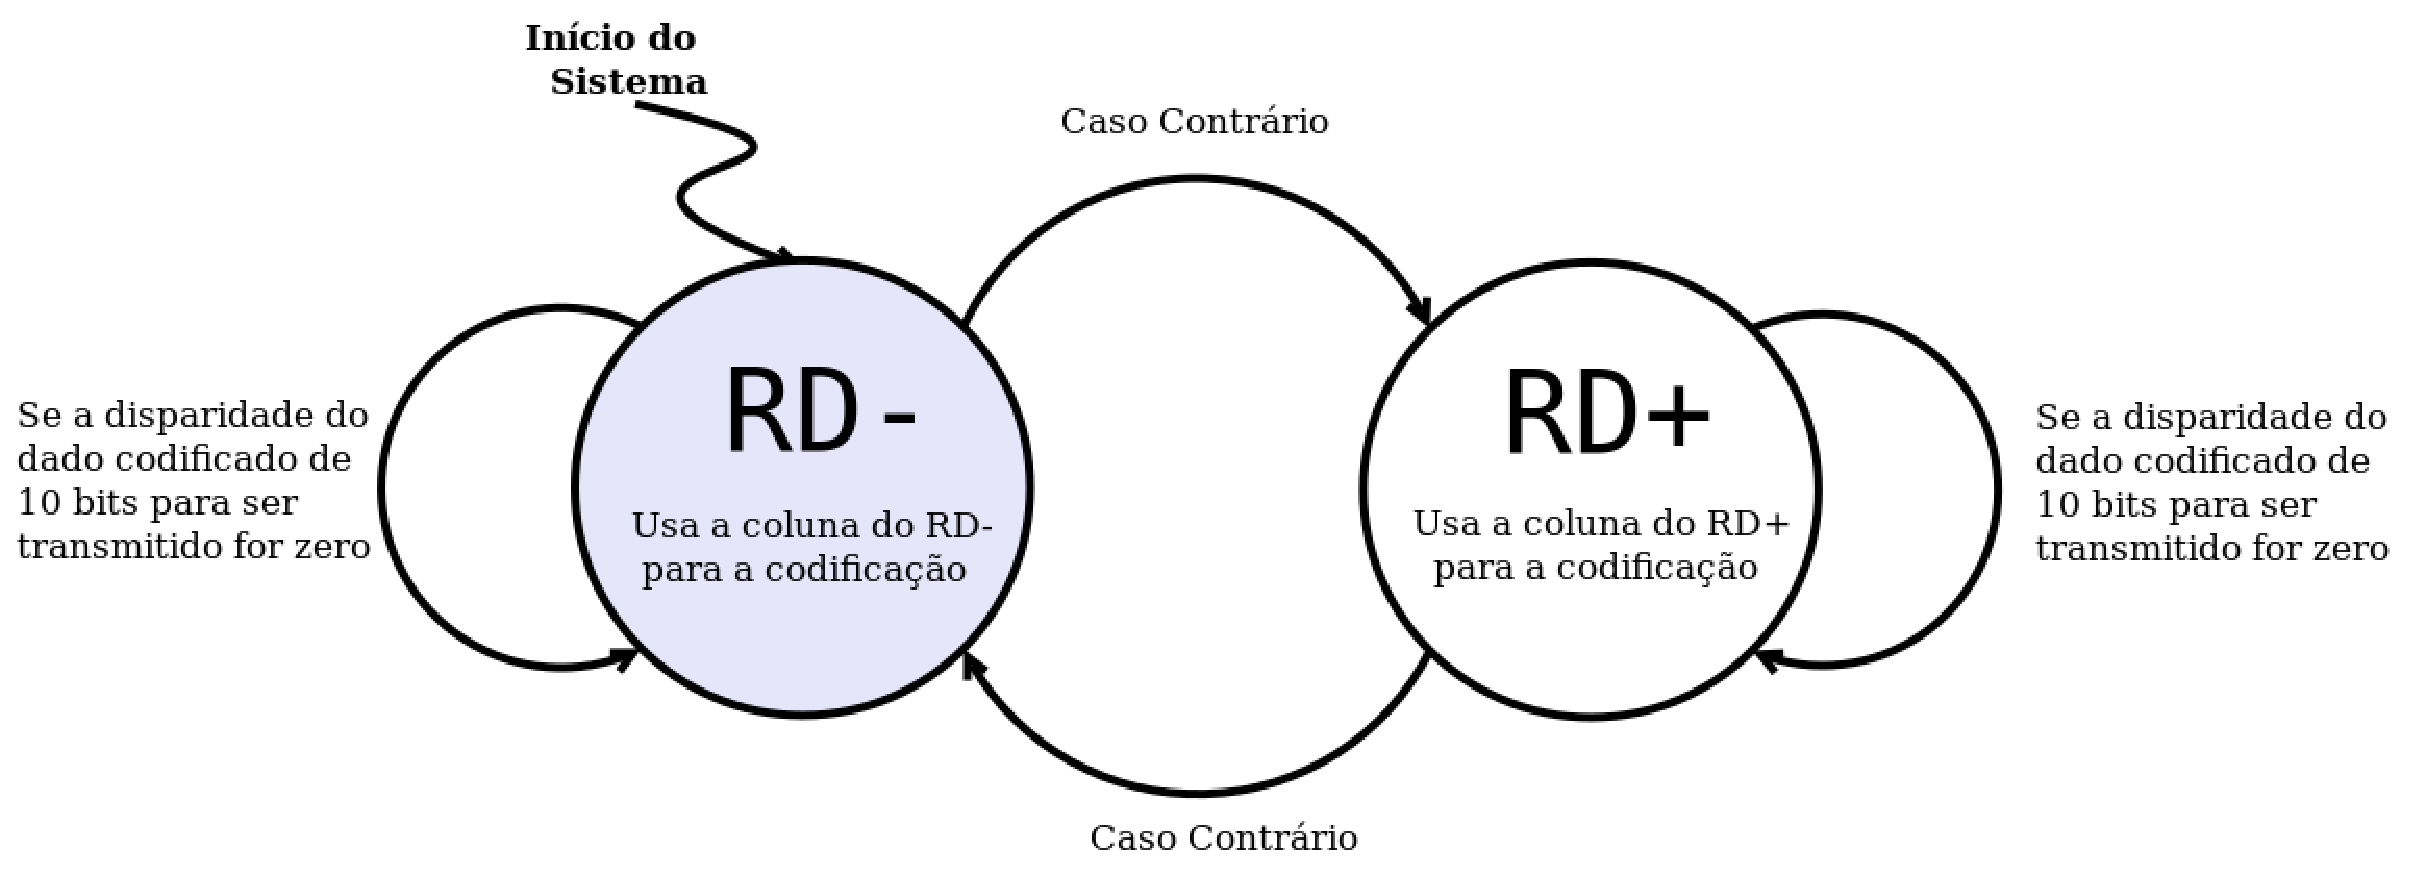
\includegraphics[scale=0.20]{esquema_rd.eps}
	\caption{Máquina de estados para a transição do RD}
	\label{rd}
\end{figure}

A característica da disparidade de dados codificados possuir sempre valores definidos (+2, -2 ou 0), possibilita a detecção de erro pelo receptor. Como descrito, para codificar os dados usa-se o RD que sempre será -1 quando o sistema for inicializado \cite{Franaszek}. Na figura \ref{coding} é ilustrado o modo como a codificação dos dados é realizada. O dado de 8 bits é separado em duas partes, codificando-os e após a sua junção é gerado um dado de 10 bits como ilustrado.  

\begin{figure}[htb]
	\centering
	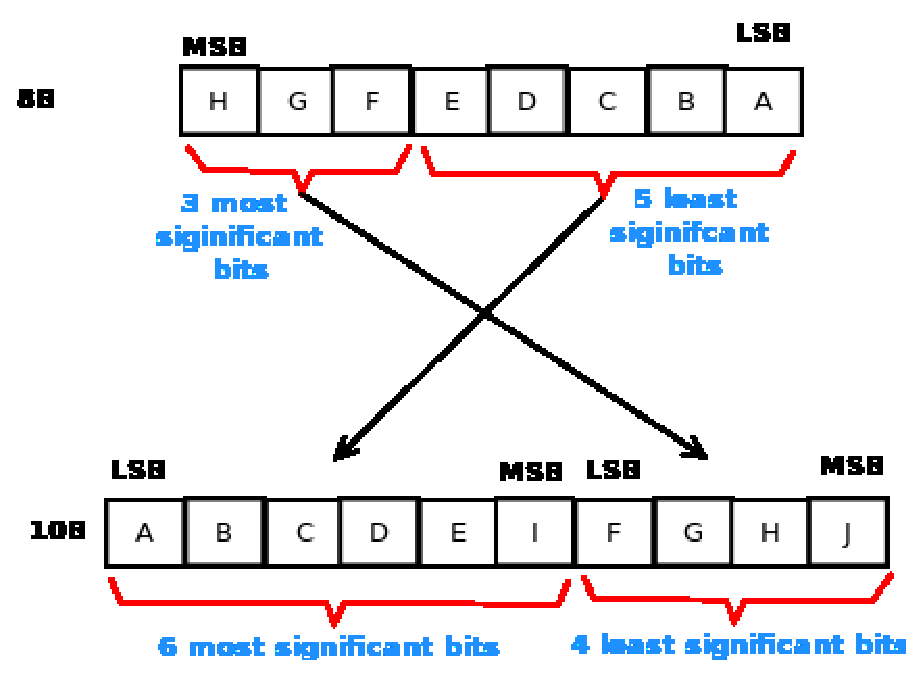
\includegraphics[scale=0.40]{coding.eps}
	\caption{Esquema da separação para codificação 8b/10b}
	\label{coding}
\end{figure}

Pela descrição, a codificação promove um balanceamento DC no sinal, ou seja, o dado a ser transmitido não possui níveis lógicos altos ou baixos por muito tempo. Esse balanço DC torna-se importante para a recuperação do relógio e consequentemente sincronização entre emissor e receptor.

\subsection{Modelagem em Máquinas de Estado da Codificação 8b/10b}

O funcionamento da codificação 8b/10b, descrita em VHDL através de máquinas de estados, é ilustrado na figura \ref{machine_system}. Como pode-se analisar há a presença de sete estados no sistema do \textit{encoder}. 

\begin{figure*}[htb]
	\centering
	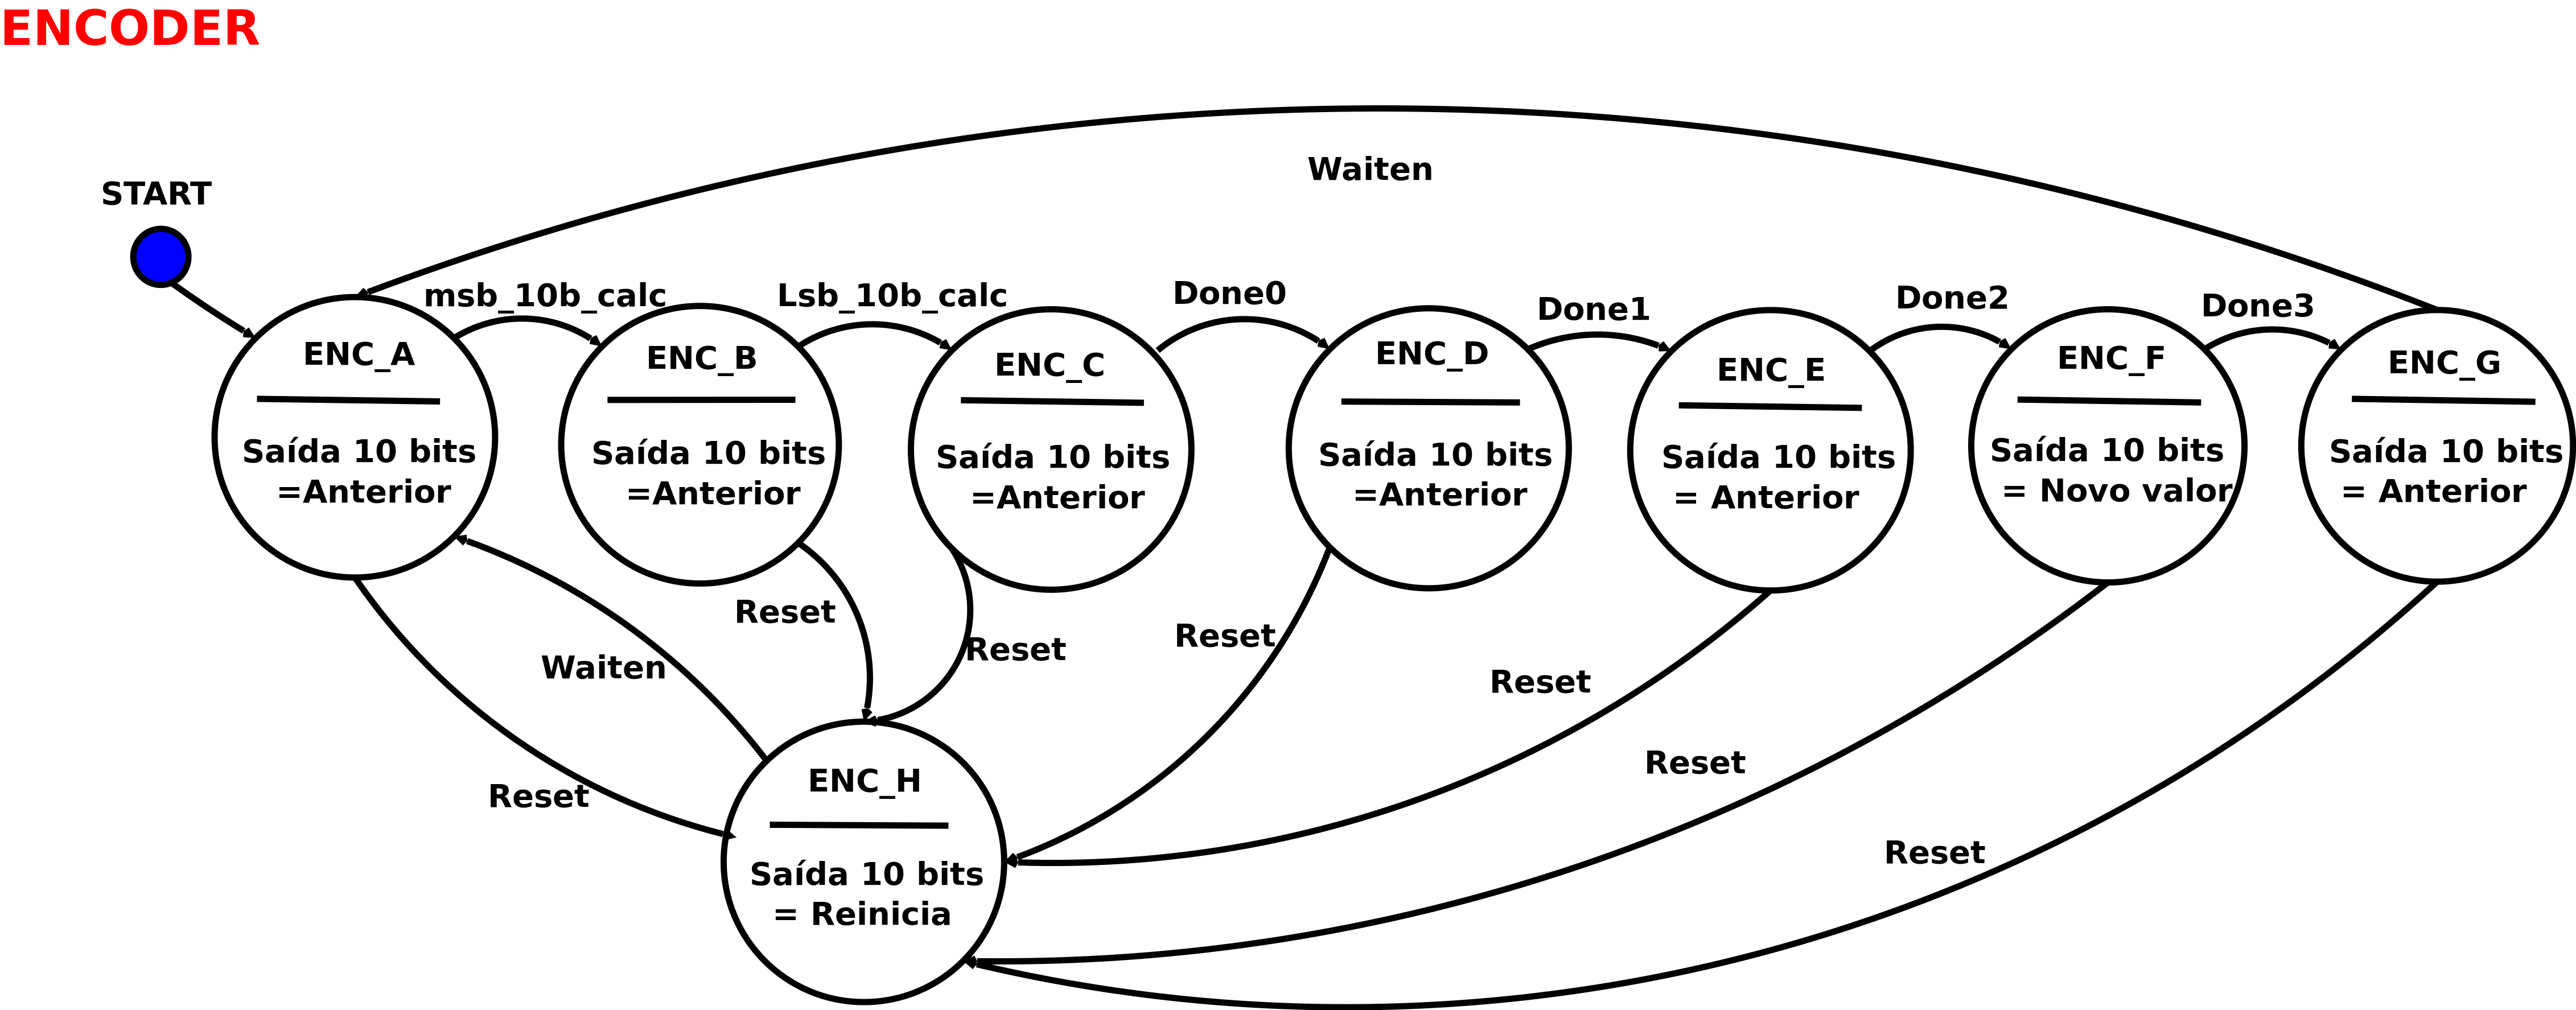
\includegraphics[scale=0.075]{FSM8b10b_v3.png}
	\caption{Máquina de estados do sistema implementado a codificação 8b/10b em VHDL}
	\label{machine_system}
\end{figure*}

No \textit{encoder} o estado "ENC\_A" refere-se ao estado de espera do dado de 8 bits na entrada. Já o estado "ENC\_B" e "ENC\_C" codificam a parte menos e mais significativas do dado de entrada (8 bits), como na figura \ref{coding}. Nos estados "ENC\_D", "ENC\_E", "ENC\_F" e "ENC\_G" realiza-se a junção das partes codificadas (saída de 10 bits), cálculo da disparidade de dados, atualização da saída e atualização do RD, respectivamente. 

A máquina de estado do \textit{decoder} apresenta comportamento similar, apesar de inverso, com o objetivo de decodificar os blocos do dado codificado. Assim a mesma é capaz de fornecer o dado de 8 bits decodificado. Caso identifique um erro, a máquina é direcionada para estados que tratam deste caso. Nestes estados, a saída vai para alta impedância, gerando um sinal de erro, e posteriormente espera-se um novo dado de entrada. 

\subsection{Descrição do Sistema da Codificação 8b/10b}
A máquina de estados foi descrita em VHDL, no software Vivado\textsuperscript{TM}, assim como o sistema para sua implementação no FPGA. Desta forma, além da descrição do \textit{encoder} e \textit{decoder}, há a necessidade de descrever todos os sistemas periféricos necessários para o funcionamento da codificação, tais como geração de dados, geração aleatória de erros, verificação de dados recebidos e sistemas de depuração 

O design FPGA proposto inclui o sistema da codificação com os demais periféricos interligados dentro de um mesmo dispositivo. O canal de transmissão entre encoder e decoder é emulado internamente no FPGA e erros podem ser inseridos arbitrariamente. A descrição do sistema para implementação no FPGA é ilustrado na figura \ref{implementation}.

\begin{figure*}[htb]
	\centering
	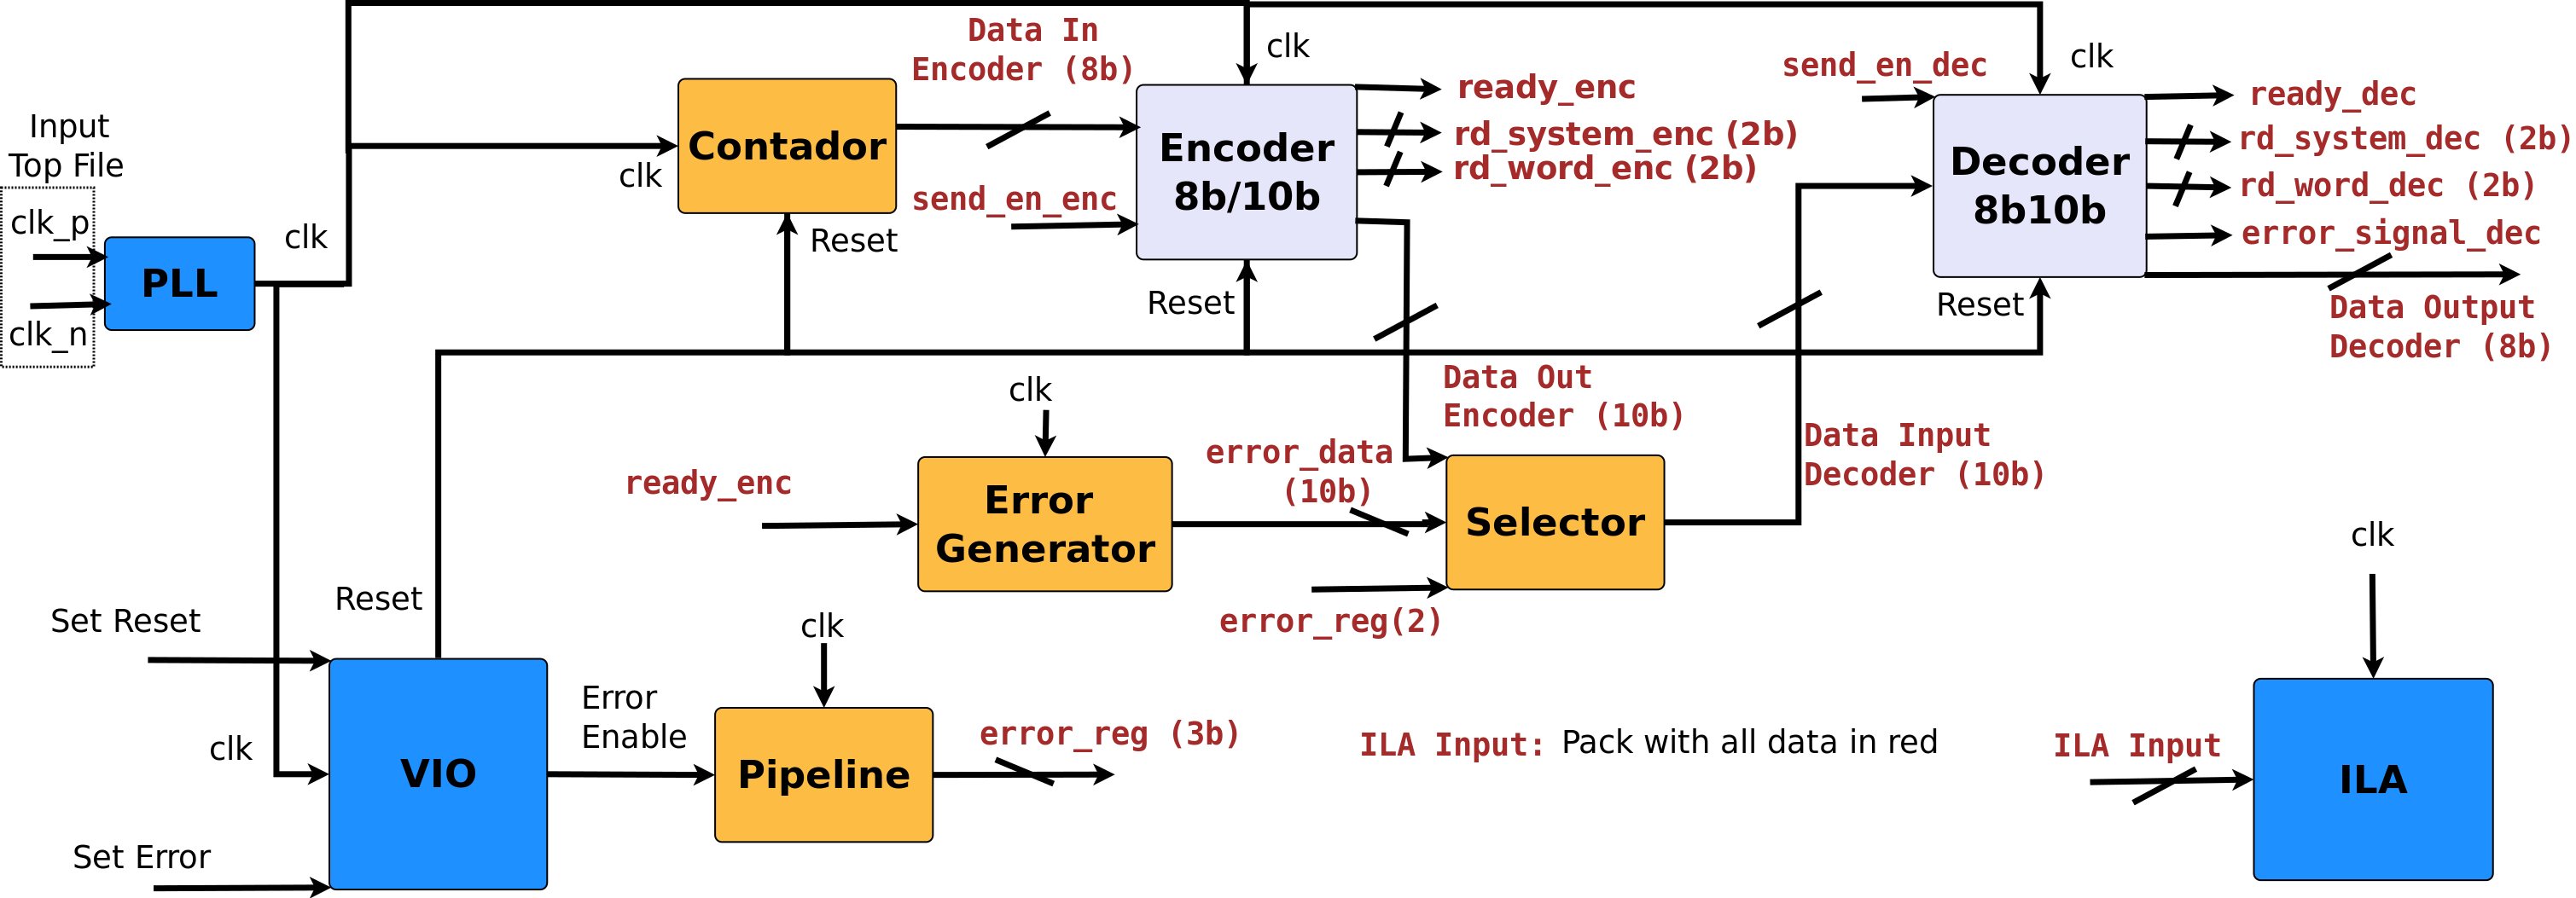
\includegraphics[scale=0.13]{hardware_system.eps}
	\caption{Descrição do Top File da codificação 8b/10b para implementação no FPGA}
	\label{implementation}
\end{figure*}

Pela figura \ref{implementation} observa-se para o funcionamento do sistema deve-se descrever um \textit{Phase-locked Loop} (PLL), um \textit{Virtual Input Output} (VIO), um \textit{Integrated Logical Analiser} (ILA), um contador para inserir dado no \textit{encoder}, um sistema (VIO, Pipeline) para inserir erro no sistema e um arranjo para modificar o dado de saída do \textit{encoder} para ser entrada no \textit{decoder}.

Através do PLL insere-se um clock de forma que o FPGA consiga implementar. O VIO permite inserir sinais dentro do sistema, já o sistema de pipeline seta um sinal de erro em somente um ciclo de \textit{clock}. O sistema \textit{Error Generator} gera um vetor de 10 bits, com apenas um bit em nível lógico alto, rotacionando-o quando o sinal \textit{ready\_enc} for alto. O bloco \textit{Selector} realiza uma operação XOR com o dado de 10 bits do \textit{Error Generator} e o dado de saída do \textit{encoder}, somente quando o sinal "error\_reg(2)" for alto. Caso contrário, o bloco seletor deixa passar somente o dado de saída do \textit{encoder}, ou seja, sem passar pela operação XOR. Pelo ILA pode-se visualizar todos os sinais dentro do sistema, dessa forma todos os dados marcados em vermelho na figura \ref{implementation} são inseridos no ILA para obter suas formas de onda.


\section{Resultados e Discussão}

Após a implementação através do software Vivado\textsuperscript{TM}, a frequência de \textit{clock} definida no teste do sistema foi de 300 MHz. 

Pelo teste da implementação obteve-se uma latência de codificação, em ciclos de \textit{clock}, de 5 ciclos até o dado de entrada estar devidamente disponível na saída. Para a decodificação, esta latência é de 4 ciclos totalizando 9 ciclos para codificação e decodificação. Porém, o sistema que insere erro na transmissão utiliza 2 ciclos de totalizando 11 ciclos para o dado codificado estar devidamente decodificado na saída.

Dessa forma, considerando uma frequência de 300 MHz a transmissão tem a capacidade de saída de dados da ordem de 480 Mbps. O ILA e VIO impedem a determinação da frequência máxima,uma vez que estes sistemas não suportaram o aumento da frequência do \textit{clock}. Dessa forma, testou-se retirar o ILA e a máxima frequência obtida foi de 400MHz, ou seja, uma taxa de dados transmitidos de 640 Mb/s. A única opção para remoção de algum componente do sistema era o ILA, pois o sistema depende do VIO para o funcionamento.

Na figura \ref{errodetected} é ilustrado a simulação do sistema no kit FPGA da Xilinx. O sinal \textit{Error Input}, gerado pelo usuário, permanecendo em nível lógico alto até que seja inserido dado no \textit{decoder} gerando erro em um bit no dado. Depois de 4 ciclos de \textit{clock}, após gerado o erro, o sistema fornece um sinal de erro. O RD entre \textit{encoder} e \textit{decoder} entra em descompasso, recuperando-se após 33 ciclos de \textit{clock}, ou seja, após 3 palavras na transmissão. 

\begin{figure*}[htb]
	\centering
	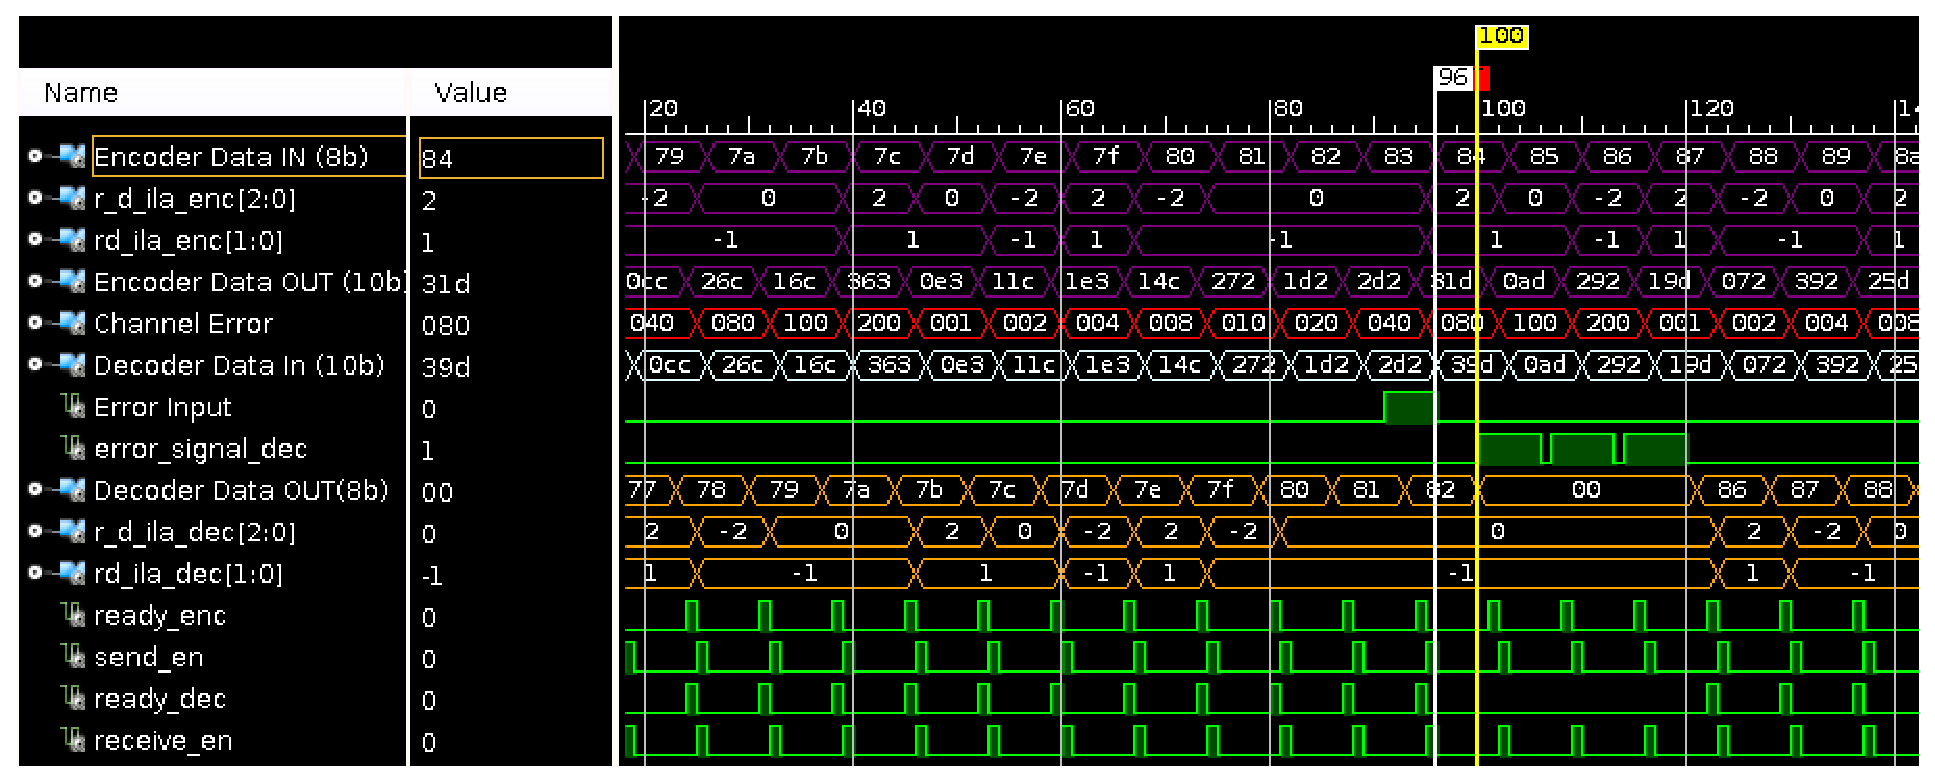
\includegraphics[scale=0.4]{error_identified.eps}
	\caption{Simulação da codificação 8b/10b implementada no FPGA com erros inseridos no canal}
	\label{errodetected}
\end{figure*}

Este descompasso do RD entre o \textit{encoder} e \textit{decoder} é característico da codificação, fazendo com que algumas palavras transmitidas sejam perdidas. Após alguns testes obteve-se um descompasso máximo de 54 ciclos, ou seja, 8 palavras perdidas na transmissão.

Emulando mais erros no canal, observou-se que o sistema,em algumas situações, decodificava o dado recebido para um valor errôneo e somente após algumas palavras o sistema sinalizava um sinal de erro. Dessa forma, é possível obter um dado válido mesmo inserindo erro, porém o sistema desbalanceia o RD ao recebê-lo. Os dados seguintes são codificados corretamente por conta de possuírem o mesmo formato para qualquer RD. Após alguns ciclos, o sistema detecta um erro por conta do desbalanço do RD. Pelos testes, a latência máxima para encontrar este erro foi de 53 ciclos.

\section{Conclusões}

A utilização de sistema codificadores para comunicação de alta velocidade é vital para sincronismos entre transmissão e recepção, bem como verificação de erros no canal. A escolha entre as codificações é realizada analisando o custo benefício entre robustez, confiabilidade, ocupação de taxa de dados e largura de banda, e qualidade do canal utilizado.

Este artigo efetuou uma implementação da codificação 8b/10b em um kit de desenvolvimento em FPGA da Xilinx (Kintex 7). Os resultados mostram que a codificação pode apresentar falha ao detectar erros, por conta do desbalanço do RD entre \textit{encoder} e \textit{decoder}. Entretanto, o sistema da codificação 8b/10b implementada no kit possui uma latência máxima de codificação e decodificação de 11 ciclos de \textit{clock}. A máxima frequência de \textit{clock} obtida pelo sistema foi de 400 MHz, com uma taxa de transferência de 480 Mb/s.

O sistema descrito e implementado no FPGA para a codificação 8b/10b, pode ser utilizado como base para a implementação e simulação no FPGA de outras codificações.   Logo este trabalho também descreve máquinas de estado para o sistema da codificação 8b/10b em VHDL. Pretende-se em trabalhos futuros, descrever um sistema que realize a análise estatística dos dados, obtendo a robustez do sistema implementado no FPGA.

\section*{Agradecimentos}

Os autores agradecem o apoio do SPRACE (Processo Fundunesp 2448/2015) e da CAPES.

\bibliographystyle{ieeetr}
\bibliography{bib-template.bib}
%%%%%%%%%%%%%%%%%%%%%%%

\end{document}